\documentclass[parskip=full]{scrartcl}

\pdfoutput=1

\title{Geometric SMOTENC \\ \LARGE{A geometrically enhanced drop-in
replacement for SMOTENC}}

\author{%
	Joao Fonseca\(^{1*}\), Fernando Bacao\(^{1}\)
	\\
	\small{\(^{1}\)NOVA Information Management School, Universidade Nova de Lisboa}
	\\
	\small{*Corresponding Author}
	\\
	\\
	\small{Postal Address: NOVA Information Management School, Campus de
    Campolide, 1070--312 Lisboa, Portugal}
	\\
	\small{Telephone: +351 21 382 8610}
}

\usepackage{breakcites}
\usepackage{float}
\usepackage{graphicx}
\usepackage{geometry}
\geometry{%
	a4paper,
	left=18mm,
	right=18mm,
	top=8mm,
}
\usepackage{amsmath}
\usepackage{enumitem}
\usepackage[ruled,vlined]{algorithm2e}
\usepackage{booktabs}
\usepackage{pgfplotstable}
\pgfplotsset{compat=1.14}
\usepackage{longtable}
\usepackage{tabu}
\usepackage{hyperref}
\date{}

\begin{document}

\maketitle

\begin{abstract}
    This is an abstract.
\end{abstract}

\section{Introduction}~\label{sec:introduction}

This is text~\cite{Chawla2002}.

\section{Related Work}~\label{sec:related_work}

\section{Motivation}~\label{sec:motivation}

$C_{maj}$ set of majority class observations (most common class found in the
target variable)

$C_{min}$ set of minority class observations (least common class found in the
target variable)


\section{Proposed Method}~\label{sec:proposed_method}

\section{Methodology}~\label{sec:methodology}

This section describes how the evaluation of G-SMOTENC was performed.  We
describe the datasets used in the experiment, their source and preprocessing
steps carried out in Section~\ref{sec:experimental_data}. We describe the
resampling and classifications methods used for comparing the performance of
G-SMOTENC with other relevant oversampling and undersampling mthods in
Section~\ref{sec:ml_algorithms}. The performance metrics used are defined in
Section~\ref{sec:performance_metrics}. Finally, the experimental procedure is
described in Section~\ref{sec:experimental_procedure}.

\subsection{Experimental Data}~\label{sec:experimental_data}

The datasets used in this experiment were extracted from the
\href{https://archive.ics.uci.edu}{UC Irvine Machine Learning Repository}. All
of the datasets are publicly available and cover a range of different domains.
The selection of datasets was done to ensure that all datasets are imbalanced
and contained non-metric features (\textit{i.e.}, whether ordinal, nominal or
binary). These datasets will be used to show how the performance of different
classifiers varies according to the used over/undersampling method.

At an initial stage, all datasets were preprocessed manually with minimal
manipulations, to avoid the application of preprocessing methods beyond the
scope of this paper. This step was conducted to remove features and/or
observations with missing values and identifying the non-metric features. The
second stage of our preprocessing was done systematically. The resulting
datasets are shown in Table~\ref{tbl:datasets_description}.

\begin{longtable}{cccccccc}
\caption{Description of the datasets collected after data preprocessing. The sampling strategy is similar across datasets. Legend: (IR) Imbalance Ratio}
\label{tbl:datasets_description}\\
\toprule
           Dataset &  Metric &  Non-Metric &  Obs. &  Min. Obs. &  Maj. Obs. &     IR &  Classes \\
\midrule
\endfirsthead
\caption[]{Description of the datasets collected after data preprocessing. The sampling strategy is similar across datasets. Legend: (IR) Imbalance Ratio} \\
\toprule
           Dataset &  Metric &  Non-Metric &  Obs. &  Min. Obs. &  Maj. Obs. &     IR &  Classes \\
\midrule
\endhead
\midrule
\multicolumn{8}{r}{{Continued on next page}} \\
\midrule
\endfoot

\bottomrule
\endlastfoot
           Abalone &       7 &           1 &  4139 &         15 &        689 &  45.93 &       18 \\
             Adult &       6 &           8 &  5000 &       1268 &       3732 &   2.94 &        2 \\
        Adult (10) &       6 &           8 &  5000 &        451 &       4549 &  10.09 &        2 \\
         Annealing &       6 &           4 &   790 &         34 &        608 &  17.88 &        4 \\
            Census &       7 &          24 &  5000 &        337 &       4663 &  13.84 &        2 \\
     Contraceptive &       5 &           4 &  1473 &        333 &        629 &   1.89 &        3 \\
Contraceptive (10) &       5 &           4 &  1036 &         62 &        629 &  10.15 &        3 \\
Contraceptive (20) &       5 &           4 &   990 &         31 &        629 &  20.29 &        3 \\
Contraceptive (31) &       5 &           4 &   973 &         20 &        629 &  31.45 &        3 \\
Contraceptive (41) &       5 &           4 &   966 &         15 &        629 &  41.93 &        3 \\
         Covertype &      10 &           2 &  5000 &         20 &       2449 & 122.45 &        7 \\
   Credit Approval &       6 &           9 &   653 &        296 &        357 &   1.21 &        2 \\
     German Credit &       7 &          13 &  1000 &        300 &        700 &   2.33 &        2 \\
German Credit (10) &       7 &          13 &   770 &         70 &        700 &  10.00 &        2 \\
German Credit (20) &       7 &          13 &   735 &         35 &        700 &  20.00 &        2 \\
German Credit (30) &       7 &          13 &   723 &         23 &        700 &  30.43 &        2 \\
German Credit (41) &       7 &          13 &   717 &         17 &        700 &  41.18 &        2 \\
     Heart Disease &       5 &           5 &   740 &         22 &        357 &  16.23 &        5 \\
Heart Disease (21) &       5 &           5 &   735 &         17 &        357 &  21.00 &        5 \\
\end{longtable}


The second part of the data preprocessing pipeline starts with the generation
of artificially imbalanced datasets with different Imbalance Ratios (IR). For
each original dataset, we create its more imbalanced versions at intervals of
10, while ensuring that $|C_{min}| \ge 15$. The sampling strategy was
determined for class $n \in \{1,\ldots,n,\ldots,m\}$ as a linear interpolation using $|C_{maj}|$ and
$|C_{min}'|=\frac{|C_{maj}|}{IR}$, as shown in equation~\ref{eq:sampling}.

\begin{equation}~\label{eq:sampling}
    |C_n|^{imb} =
    \frac{\frac{|C_{maj}|}{IR}-|C_{maj}|}{|\{1,\ldots,n,\ldots,m\}|-1}.|C_n|+|C_{max}|
\end{equation}

The new, artificially imbalanced dataset, is formed by randomly removing
observations from each $C_n$ such that $C_n' \subseteq C_n , |C_n'| =
|C_n|^{imb}$. The artificially imbalanced datasets are marked with its
imbalance ratio as a suffix in Table~\ref{tbl:datasets_description}.

The datasets (both original and artificially imbalanced versions) are then
filtered to ensure all datasets have a minimum of 500 observations.  The
remaining datasets whose number of observations is larger than 5000 are
randomly sampled to match this number of observations. Afterwards, for each
remaining dataset we remove all observations from target classes whose
frequency is lower than 15 observations. Finally, the continuous and discrete
features are scaled to the range $[0,1]$ to ensure a common range between all
features. 

\subsection{Machine Learning Algorithms}~\label{sec:ml_algorithms}

The choice of classifiers used in the experimental procedure were based on
their type (tree-based, nearest neighbors-based, linear model and
ensemble-based), popularity and consistency in performance. We used Decision
Tree (DT), a K-Nearest Neighbors (KNN) classifier, a Logistic
Regression (LR) and a Random Forest (RF).

Given the lack of existing oversamplers that address imbalanced learning
problems with mixed data types, the amount of benchmark methods used is also
limited. We used the well known methods that are compatible with this type of
datasets: SMOTENC, Random Undersampling (RUS) and Random Oversampling (ROS).
Table~\ref{tbl:grid} shows the hyperparameters used for the parameter search
described in Section~\ref{sec:experimental_procedure}.

\begin{table}
	\centering
    \caption{\label{tbl:grid}
        Hyperparameter definition for the classifiers and resamplers used in
        the experiment.
    }
	\begin{tabular}{lll}
		\toprule
		Classifier      &                                  &                                \\
		\midrule
        DT              & min.\ samples split              & 2                              \\
                        & criterion                        & gini                           \\
                        & max depth                        & 3, 6                           \\
		LR              & maximum iterations               & 10000                          \\
                        & multi-class                      & One-vs-All                     \\
		                & solver                           & saga                           \\
                        & penalty                          & None, L1, L2                   \\
		KNN             & \# neighbors                     & 3, 5                           \\
                        & weights                          & uniform                        \\
                        & metric                           & euclidean                      \\
		RF              & min.\ samples split              & 2                              \\
		                & \# estimators                    & 50, 100                        \\
		                & Max depth                        & 3, 6                           \\
                        & criterion                        & gini                           \\
		\toprule
		Resampler       &                                  &                                \\
		\midrule
		SMOTENC         & \# neighbors                     & 3, 5                           \\
		G-SMOTENC       & \# neighbors                     & 3, 5                           \\
                        & deformation factor               & 0.0, 0.25, 0.5, 0.75, 1.0      \\
                        & truncation factor                & -1.0, -0.5, 0.0, 0.5, 1.0      \\
                        & selection strategy               & ``combined'',
                        ``minority'', ``majority''\\
		RUS             & replacement                      & False                          \\
		ROS             & (no applicable parameters)       &                                \\
		\bottomrule
	\end{tabular}
\end{table}

\subsection{Performance Metrics}~\label{sec:performance_metrics}

Although the typical performance metrics, \textit{e.g.}, Overall Accuracy
(OA), are intuitive to interpret, they are often inappropriate to measure a
classifier's performance in an imbalanced learning context
\textbf{[CITATION]}. For example, to estimate an event that occurs in 1\% of
the dataset, a constant classifier would obtain an OA of 0.99 and still be
unusable. However, this metric is still reported in some of our results to
maintain a metric that is easier to interpret.

More recent surveys have found the Geometric-mean ($\textit{G-mean} =
\sqrt{\overline{Sensitivity} \times \overline{Specificity}}$), F1-score
($\textit{F-score}=2\times\frac{\overline{Precision} \times
\overline{Recall}}{\overline{Precision} + \overline{Recall}}$), $Sensitivity =
\frac{TP}{FN+TP}$ and $Specificity = \frac{TN}{TN + FP}$ to be commonly used
performance metrics in imbalanced learning contexts~\cite{rout2018handling}.
These metrics are calculated as a function of the number of False/True
Positives (FP and TP) and False/True Negatives (FN and TN), having
$Precision = \frac{TP}{TP+FP}$ and $Recall = \frac{TP}{TP+FN}$.
This finding is consistent with other well-known recommendations on the usage
of performance metrics~\cite{jeni2013facing}. This led us to adopt, along with
OA, both F-score and G-mean as the main performance metrics for this study. 

\subsection{Experimental Procedure}~\label{sec:experimental_procedure}

The experimental procedure was applied similarly to all combinations of
resamplers, classifiers and hyperparameter combinations across all datasets.
The evaluation of the models' performance was tested using a 5-fold Cross
Validation (CV) approach. The mean performance in the test set is calculated
over the 5 folds and 3 different runs of the experimental procedure for each
combination resampling/classifier hyperparameters. For each dataset, results
of the hyperparameters that optimize the performance of a resampler/classifier
are selected. These results were then used for analysis and are shown in
Table~\ref{tbl:wide_optimal} (see Appendix).
Figure~\ref{fig:experimental_procedure} shows a diagram of the experimental
procedure described.

\begin{figure}
	\centering
	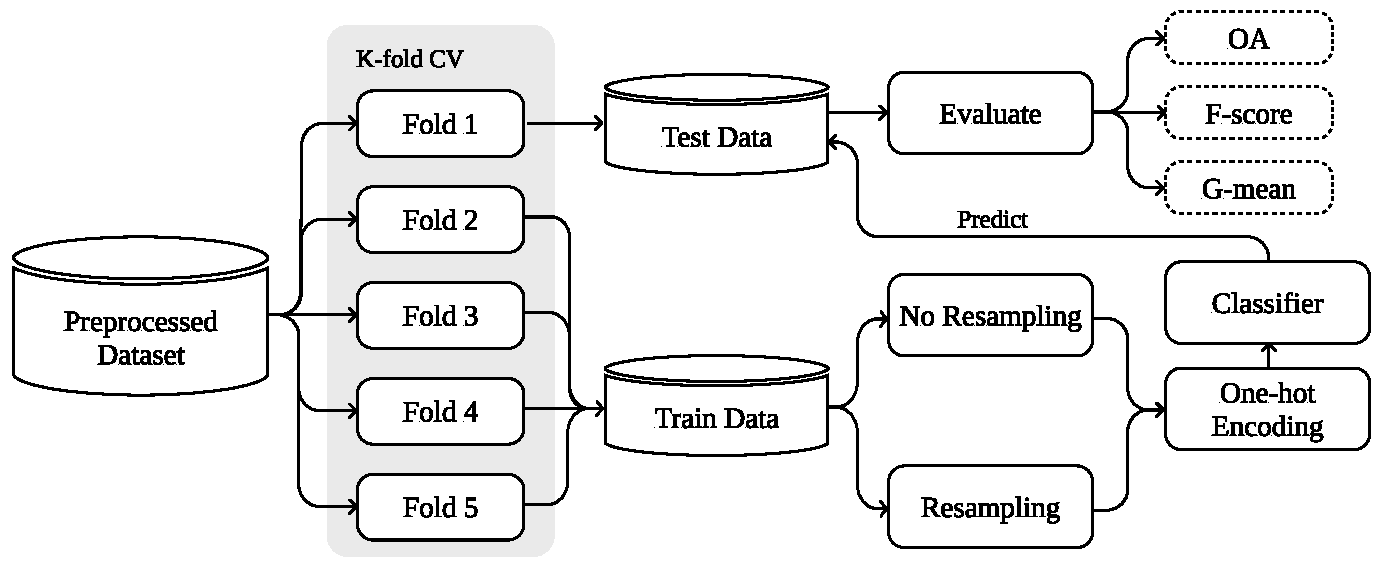
\includegraphics[width=.8\linewidth]{../analysis/experimental_procedure}
    \caption{Experimental procedure used in this study.
    }~\label{fig:experimental_procedure}
\end{figure}

A CV run consists of a stratified partitioning (\textit{i.e.}, each partition
contains the same relative frequencies of target labels) of the dataset into
five parts. A given resampler/classifier combination with a specific set of
hyperparameters is fit and tested five times, using one of the partitions as a
test set and the remaining ones as training set. The estimated performance
consists of the average classification performance across the five different
test sets. 

\subsection{Software Implementation}~\label{sec:software_implementation}

The algorithmic implementation of G-SMOTENC was written using the Python
programming language and is available in the open-source package
\href{https://github.com/joaopfonseca/ml-research}{ML-Research}~\cite{fonseca2021increasing},
along with other utilities used to produce the experiment and outputs used in
Section~\ref{sec:results_and_discussion}. In addition, the packages
\href{https://github.com/scikit-learn/scikit-learn/}{Scikit-Learn}~\cite{scikit-learn},
\href{https://github.com/scikit-learn-contrib/imbalanced-learn}{Imbalanced-Learn}~\cite{JMLR:v18:16-365}
and \href{https://github.com/georgedouzas/research-learn/}{Research-Learn}
were also used in the experimental procedure to get the implementations of the
classifiers, benchmark over/undersamplers and run the experimental procedure.
The Latex code, Python scripts (including data pulling and preprocessing,
experiment setup and results' analysis), as well as the datasets used are
available in this \href{https://github.com/joaopfonseca/publications}{GitHub
repository}.
 

\section{Results and Discussion}~\label{sec:results_and_discussion}

In this section we present the experimental results. We focus on the
comparison of classification performance using oversamplers whose generation
mechanism is compatible with datasets containing both continuous and
categorical features.

The analysis of our experimental results were developed in two stages: (1)
analysis of mean ranking and absolute performance and (2) statistical
analysis. In Section~\ref{sec:discussion} we discuss the main insights
extracted by analysing the results reported in Sections~\ref{sec:results}
and~\ref{sec:statistical_analysis}.

\subsection{Results}~\label{sec:results}

Table~\ref{tbl:mean_sem_ranks} presents the mean rankings of cross validation
scores across the different combinations of oversamplers, metrics and
classifiers. These results were calculated by assigning a ranking score for
each oversampler from 1 (best) to 4 (worst) for each dataset, metric and
classifier, based on the results reported in Table~\ref{tbl:wide_optimal} (see
Appendix).

\begin{longtable}{ccccccc}
\caption{Mean rankings over the different datasets, folds and runs used in the experiment.}
\label{tbl:mean_sem_ranks}\\
\toprule
Classifier &  Metric &                G-SMOTENC &                     NONE &         SMOTENC &                      ROS &             RUS \\
\midrule
\endfirsthead
\caption[]{Mean rankings over the different datasets, folds and runs used in the experiment.} \\
\toprule
Classifier &  Metric &                G-SMOTENC &                     NONE &         SMOTENC &                      ROS &             RUS \\
\midrule
\endhead
\midrule
\multicolumn{7}{r}{{Continued on next page}} \\
\midrule
\endfoot

\bottomrule
\endlastfoot
        DT &      OA &          1.66 $\pm$ 0.13 & \textbf{1.55 $\pm$ 0.22} & 3.16 $\pm$ 0.16 &          4.00 $\pm$ 0.08 & 4.63 $\pm$ 0.19 \\
        DT & F-Score & \textbf{1.11 $\pm$ 0.07} &          3.21 $\pm$ 0.30 & 2.58 $\pm$ 0.18 &          3.53 $\pm$ 0.16 & 4.58 $\pm$ 0.19 \\
        DT &  G-Mean & \textbf{1.53 $\pm$ 0.21} &          4.89 $\pm$ 0.07 & 2.53 $\pm$ 0.18 &          2.47 $\pm$ 0.23 & 3.58 $\pm$ 0.23 \\
       KNN &      OA &          2.39 $\pm$ 0.12 & \textbf{1.32 $\pm$ 0.23} & 3.58 $\pm$ 0.16 &          2.97 $\pm$ 0.26 & 4.74 $\pm$ 0.17 \\
       KNN & F-Score & \textbf{1.37 $\pm$ 0.16} &          3.37 $\pm$ 0.28 & 2.68 $\pm$ 0.20 &          2.95 $\pm$ 0.27 & 4.63 $\pm$ 0.17 \\
       KNN &  G-Mean & \textbf{1.74 $\pm$ 0.17} &          4.84 $\pm$ 0.12 & 2.63 $\pm$ 0.17 &          3.26 $\pm$ 0.25 & 2.53 $\pm$ 0.35 \\
        LR &      OA &          2.47 $\pm$ 0.15 & \textbf{1.32 $\pm$ 0.23} & 2.76 $\pm$ 0.17 &          3.66 $\pm$ 0.21 & 4.79 $\pm$ 0.16 \\
        LR & F-Score & \textbf{1.89 $\pm$ 0.21} &          3.84 $\pm$ 0.28 & 2.05 $\pm$ 0.24 &          2.79 $\pm$ 0.25 & 4.42 $\pm$ 0.21 \\
        LR &  G-Mean &          1.97 $\pm$ 0.23 &          5.00 $\pm$ 0.00 & 3.29 $\pm$ 0.17 & \textbf{1.89 $\pm$ 0.17} & 2.84 $\pm$ 0.30 \\
        RF &      OA &          1.76 $\pm$ 0.09 & \textbf{1.24 $\pm$ 0.09} & 3.37 $\pm$ 0.11 &          3.66 $\pm$ 0.12 & 4.97 $\pm$ 0.03 \\
        RF & F-Score & \textbf{1.26 $\pm$ 0.13} &          4.21 $\pm$ 0.25 & 2.68 $\pm$ 0.17 &          2.42 $\pm$ 0.22 & 4.42 $\pm$ 0.12 \\
        RF &  G-Mean & \textbf{1.68 $\pm$ 0.22} &          4.84 $\pm$ 0.16 & 2.89 $\pm$ 0.21 &          2.26 $\pm$ 0.23 & 3.32 $\pm$ 0.25 \\
\end{longtable}


Table~\ref{tbl:mean_sem_scores} presents the mean cross validation scores.
With exception to the OA metric, G-SMOTENC either outperformed or matched the
the remaining oversamplers.

\begin{longtable}{ccccccc}
\caption{Mean scores over the different datasets, folds and runs used in the experiment}
\label{tbl:mean_sem_scores}\\
\toprule
Classifier &  Metric &                  G-SMOTE &                     NONE &                  SMOTENC &                      ROS &             RUS \\
\midrule
\endfirsthead
\caption[]{Mean scores over the different datasets, folds and runs used in the experiment} \\
\toprule
Classifier &  Metric &                  G-SMOTE &                     NONE &                  SMOTENC &                      ROS &             RUS \\
\midrule
\endhead
\midrule
\multicolumn{7}{r}{{Continued on next page}} \\
\midrule
\endfoot

\bottomrule
\endlastfoot
        DT &      OA &          0.74 $\pm$ 0.04 & \textbf{0.75 $\pm$ 0.04} &          0.68 $\pm$ 0.04 &          0.66 $\pm$ 0.04 & 0.58 $\pm$ 0.04 \\
        DT & F-Score & \textbf{0.56 $\pm$ 0.04} &          0.52 $\pm$ 0.04 &          0.54 $\pm$ 0.04 &          0.52 $\pm$ 0.04 & 0.48 $\pm$ 0.04 \\
        DT &  G-Mean & \textbf{0.69 $\pm$ 0.02} &          0.60 $\pm$ 0.02 &          0.68 $\pm$ 0.03 &          0.67 $\pm$ 0.03 & 0.65 $\pm$ 0.03 \\
       KNN &      OA &          0.69 $\pm$ 0.04 & \textbf{0.73 $\pm$ 0.05} &          0.67 $\pm$ 0.04 &          0.69 $\pm$ 0.05 & 0.57 $\pm$ 0.04 \\
       KNN & F-Score & \textbf{0.53 $\pm$ 0.04} &          0.50 $\pm$ 0.04 &          0.52 $\pm$ 0.04 &          0.52 $\pm$ 0.04 & 0.46 $\pm$ 0.04 \\
       KNN &  G-Mean & \textbf{0.66 $\pm$ 0.03} &          0.58 $\pm$ 0.02 &          0.64 $\pm$ 0.03 &          0.62 $\pm$ 0.03 & 0.65 $\pm$ 0.03 \\
        LR &      OA &          0.68 $\pm$ 0.04 & \textbf{0.75 $\pm$ 0.04} &          0.68 $\pm$ 0.05 &          0.66 $\pm$ 0.04 & 0.58 $\pm$ 0.04 \\
        LR & F-Score & \textbf{0.54 $\pm$ 0.04} &          0.52 $\pm$ 0.04 & \textbf{0.54 $\pm$ 0.04} &          0.53 $\pm$ 0.04 & 0.48 $\pm$ 0.04 \\
        LR &  G-Mean & \textbf{0.69 $\pm$ 0.02} &          0.60 $\pm$ 0.02 &          0.68 $\pm$ 0.02 & \textbf{0.69 $\pm$ 0.02} & 0.67 $\pm$ 0.03 \\
        RF &      OA &          0.74 $\pm$ 0.04 & \textbf{0.76 $\pm$ 0.04} &          0.69 $\pm$ 0.04 &          0.69 $\pm$ 0.04 & 0.59 $\pm$ 0.04 \\
        RF & F-Score & \textbf{0.57 $\pm$ 0.04} &          0.48 $\pm$ 0.04 &          0.55 $\pm$ 0.04 &          0.55 $\pm$ 0.04 & 0.49 $\pm$ 0.04 \\
        RF &  G-Mean & \textbf{0.70 $\pm$ 0.02} &          0.57 $\pm$ 0.02 &          0.68 $\pm$ 0.03 &          0.69 $\pm$ 0.03 & 0.68 $\pm$ 0.03 \\
\end{longtable}


\subsection{Statistical Analysis}~\label{sec:statistical_analysis}

Based on the literature found, in Section~\ref{sec:performance_metrics} we
explained that OA, although easily interpretable, is not an appropriate
performance metric for imbalanced learning problems. Therefore, the
statistical analysis was developed using the two imbalance-appropriate metrics
used in the study: F-Score and G-Mean. The statistical analysis started with
the assessment of a statistically significant difference in performance across
resampling methods using a Friedman test~\cite{friedman1937use}. The results
of this test are shown in Table~\ref{tbl:friedman_test}.

\begin{longtable}{cccc}
\caption{Results for the Friedman test. Statistical significance is tested at a level of $\alpha = 0.05$. The null hypothesis is that there is no difference in the classification outcome across resamplers.}
\label{tbl:friedman_test}\\
\toprule
Classifier &  Metric & p-value &  Significance \\
\midrule
\endfirsthead
\caption[]{Results for the Friedman test. Statistical significance is tested at a level of $\alpha = 0.05$. The null hypothesis is that there is no difference in the classification outcome across resamplers.} \\
\toprule
Classifier &  Metric & p-value &  Significance \\
\midrule
\endhead
\midrule
\multicolumn{4}{r}{{Continued on next page}} \\
\midrule
\endfoot

\bottomrule
\endlastfoot
        DT & F-Score & 2.2e-10 &          True \\
        DT &  G-Mean & 1.2e-10 &          True \\
       KNN & F-Score & 2.3e-09 &          True \\
       KNN &  G-Mean & 9.4e-10 &          True \\
        LR & F-Score & 2.1e-07 &          True \\
        LR &  G-Mean & 9.7e-11 &          True \\
        RF & F-Score & 8.5e-12 &          True \\
        RF &  G-Mean & 2.0e-10 &          True \\
\end{longtable}


\begin{longtable}{ccccccc}
\caption{Adjusted p-values using the Holm-Bonferroni test. Statistical significance is tested at a level of $\alpha = 0.05$. The null hypothesis is that the benchmark methods perform similarly compared to the control method (G-SMOTENC).}
\label{tbl:holms_test}\\
\toprule
Classifier &  Metric &               NONE &            SMOTENC &                ROS &                RUS &          SMOTE-ENC \\
\midrule
\endfirsthead
\caption[]{Adjusted p-values using the Holm-Bonferroni test. Statistical significance is tested at a level of $\alpha = 0.05$. The null hypothesis is that the benchmark methods perform similarly compared to the control method (G-SMOTENC).} \\
\toprule
Classifier &  Metric &               NONE &            SMOTENC &                ROS &                RUS &          SMOTE-ENC \\
\midrule
\endhead
\midrule
\multicolumn{7}{r}{{Continued on next page}} \\
\midrule
\endfoot

\bottomrule
\endlastfoot
        DT & F-Score & \textbf{{1.5e-04}} & \textbf{{1.5e-04}} & \textbf{{7.3e-06}} & \textbf{{1.2e-06}} &          {1.0e-01} \\
        DT &  G-Mean & \textbf{{5.6e-07}} & \textbf{{2.7e-03}} & \textbf{{2.8e-02}} & \textbf{{3.9e-04}} & \textbf{{2.3e-02}} \\
       KNN & F-Score & \textbf{{6.4e-04}} & \textbf{{2.2e-04}} & \textbf{{7.2e-04}} & \textbf{{6.4e-04}} & \textbf{{5.9e-06}} \\
       KNN &  G-Mean & \textbf{{1.6e-05}} & \textbf{{9.6e-03}} & \textbf{{6.5e-03}} &          {2.0e-01} & \textbf{{3.5e-03}} \\
        LR & F-Score & \textbf{{4.0e-03}} &          {6.1e-01} & \textbf{{9.2e-03}} & \textbf{{3.6e-04}} &          {5.6e-02} \\
        LR &  G-Mean & \textbf{{1.6e-07}} & \textbf{{4.0e-04}} &          {8.6e-01} &          {2.4e-01} & \textbf{{4.7e-03}} \\
        RF & F-Score & \textbf{{1.7e-06}} & \textbf{{2.4e-04}} & \textbf{{8.0e-03}} & \textbf{{1.7e-06}} & \textbf{{8.0e-03}} \\
        RF &  G-Mean & \textbf{{3.8e-06}} & \textbf{{8.8e-03}} &          {2.5e-01} & \textbf{{2.3e-02}} & \textbf{{1.7e-03}} \\
\end{longtable}


\subsection{Discussion}~\label{sec:discussion}

\begin{figure}
	\centering
	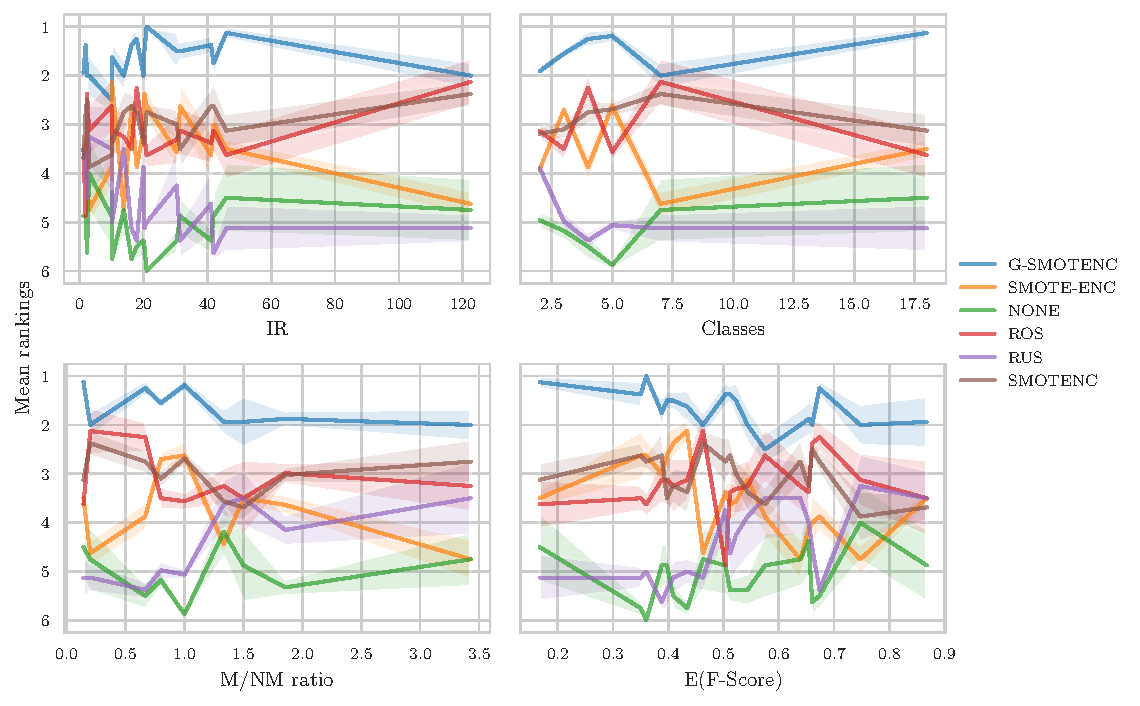
\includegraphics[width=\linewidth]{../analysis/consistency_analysis_plot}
    \caption{Average ranking of oversamplers over different characteristics of
        the datasets used in the experiment. Legend: IR --- Imbalance Ratio,
        Classes --- Number of classes in the dataset, M/NM ratio --- ratio
        between the number of metric and non-metric features, E$($F-Score$)$
        --- Mean F-Score of dataset across all combinations of classifiers and
        oversamplers.
    }~\label{fig:consistency_analysis}
\end{figure}

\section{Conclusion}~\label{sec:conclusion}

\bibliography{references}
\bibliographystyle{ieeetr}

\appendix

\section{Appendix}

\begin{longtable}{cccccccc}
\caption{Wide optimal results}
\label{tbl:wide_optimal}\\
\toprule
           Dataset & Classifier &  Metric &      G-SMOTENC &           NONE &        SMOTENC &            ROS &            RUS \\
\midrule
\endfirsthead
\caption[]{Wide optimal results} \\
\toprule
           Dataset & Classifier &  Metric &      G-SMOTENC &           NONE &        SMOTENC &            ROS &            RUS \\
\midrule
\endhead
\midrule
\multicolumn{8}{r}{{Continued on next page}} \\
\midrule
\endfoot

\bottomrule
\endlastfoot
           Abalone &         DT &      OA &          0.221 & \textbf{0.256} &          0.190 &          0.203 &          0.207 \\
           Abalone &         DT & F-Score &          0.168 & \textbf{0.170} &          0.156 &          0.154 &          0.132 \\
           Abalone &         DT &  G-Mean & \textbf{0.460} &          0.413 &          0.445 &          0.457 &          0.421 \\
           Abalone &        KNN &      OA &          0.215 & \textbf{0.237} &          0.186 &          0.197 &          0.188 \\
           Abalone &        KNN & F-Score & \textbf{0.167} &          0.157 &          0.150 &          0.151 &          0.140 \\
           Abalone &        KNN &  G-Mean & \textbf{0.429} &          0.391 &          0.409 &          0.397 &          0.421 \\
           Abalone &         LR &      OA &          0.235 & \textbf{0.272} &          0.228 &          0.229 &          0.195 \\
           Abalone &         LR & F-Score & \textbf{0.189} &          0.180 &          0.186 &          0.179 &          0.166 \\
           Abalone &         LR &  G-Mean & \textbf{0.473} &          0.415 &          0.466 &          0.456 &          0.441 \\
           Abalone &         RF &      OA &          0.237 & \textbf{0.276} &          0.221 &          0.224 &          0.197 \\
           Abalone &         RF & F-Score & \textbf{0.194} &          0.174 &          0.180 &          0.184 &          0.162 \\
           Abalone &         RF &  G-Mean & \textbf{0.486} &          0.416 &          0.461 &          0.465 &          0.448 \\
             Adult &         DT &      OA &          0.830 & \textbf{0.835} &          0.785 &          0.800 &          0.785 \\
             Adult &         DT & F-Score & \textbf{0.767} &          0.763 &          0.754 &          0.755 &          0.744 \\
             Adult &         DT &  G-Mean & \textbf{0.809} &          0.747 &          0.808 &          0.806 &          0.801 \\
             Adult &        KNN &      OA &          0.786 & \textbf{0.805} &          0.781 &          0.763 &          0.761 \\
             Adult &        KNN & F-Score & \textbf{0.738} &          0.732 &          0.735 &          0.718 &          0.728 \\
             Adult &        KNN &  G-Mean &          0.766 &          0.724 &          0.762 &          0.757 & \textbf{0.780} \\
             Adult &         LR &      OA &          0.803 & \textbf{0.839} &          0.803 &          0.804 &          0.801 \\
             Adult &         LR & F-Score &          0.768 & \textbf{0.773} &          0.767 &          0.771 &          0.769 \\
             Adult &         LR &  G-Mean &          0.813 &          0.758 &          0.805 & \textbf{0.815} & \textbf{0.815} \\
             Adult &         RF &      OA &          0.820 & \textbf{0.832} &          0.757 &          0.755 &          0.753 \\
             Adult &         RF & F-Score & \textbf{0.769} &          0.739 &          0.727 &          0.729 &          0.728 \\
             Adult &         RF &  G-Mean &          0.796 &          0.711 &          0.787 & \textbf{0.797} & \textbf{0.797} \\
        Adult (10) &         DT &      OA & \textbf{0.930} &          0.928 &          0.822 &          0.789 &          0.775 \\
        Adult (10) &         DT & F-Score & \textbf{0.711} &          0.708 &          0.656 &          0.641 &          0.630 \\
        Adult (10) &         DT &  G-Mean &          0.812 &          0.663 &          0.807 & \textbf{0.815} &          0.808 \\
        Adult (10) &        KNN &      OA &          0.864 & \textbf{0.909} &          0.854 &          0.851 &          0.745 \\
        Adult (10) &        KNN & F-Score & \textbf{0.667} &          0.652 &          0.658 &          0.648 &          0.602 \\
        Adult (10) &        KNN &  G-Mean &          0.745 &          0.629 &          0.747 &          0.722 & \textbf{0.783} \\
        Adult (10) &         LR &      OA &          0.836 & \textbf{0.925} &          0.837 &          0.815 &          0.791 \\
        Adult (10) &         LR & F-Score &          0.666 & \textbf{0.705} &          0.667 &          0.663 &          0.647 \\
        Adult (10) &         LR &  G-Mean &          0.804 &          0.663 &          0.787 &          0.811 & \textbf{0.814} \\
        Adult (10) &         RF &      OA &          0.899 & \textbf{0.924} &          0.773 &          0.763 &          0.743 \\
        Adult (10) &         RF & F-Score & \textbf{0.718} &          0.615 &          0.620 &          0.624 &          0.610 \\
        Adult (10) &         RF &  G-Mean & \textbf{0.809} &          0.579 &          0.786 &          0.806 &          0.806 \\
         Annealing &         DT &      OA &          0.824 & \textbf{0.843} &          0.742 &          0.733 &          0.694 \\
         Annealing &         DT & F-Score & \textbf{0.736} &          0.643 &          0.732 &          0.724 &          0.683 \\
         Annealing &         DT &  G-Mean & \textbf{0.914} &          0.738 &          0.909 &          0.906 &          0.880 \\
         Annealing &        KNN &      OA &          0.849 &          0.847 &          0.829 & \textbf{0.854} &          0.508 \\
         Annealing &        KNN & F-Score &          0.780 &          0.724 &          0.747 & \textbf{0.783} &          0.476 \\
         Annealing &        KNN &  G-Mean &          0.901 &          0.781 &          0.867 & \textbf{0.909} &          0.814 \\
         Annealing &         LR &      OA &          0.572 & \textbf{0.814} &          0.573 &          0.566 &          0.510 \\
         Annealing &         LR & F-Score & \textbf{0.620} &          0.540 &          0.617 &          0.615 &          0.496 \\
         Annealing &         LR &  G-Mean & \textbf{0.851} &          0.663 &          0.843 &          0.848 &          0.811 \\
         Annealing &         RF &      OA & \textbf{0.868} & \textbf{0.868} &          0.729 &          0.733 &          0.637 \\
         Annealing &         RF & F-Score & \textbf{0.800} &          0.644 &          0.730 &          0.736 &          0.641 \\
         Annealing &         RF &  G-Mean & \textbf{0.917} &          0.727 &          0.904 &          0.910 &          0.873 \\
            Census &         DT &      OA &          0.942 & \textbf{0.943} &          0.894 &          0.844 &          0.795 \\
            Census &         DT & F-Score & \textbf{0.733} &          0.731 &          0.693 &          0.652 &          0.617 \\
            Census &         DT &  G-Mean &          0.813 &          0.698 &          0.800 &          0.814 & \textbf{0.817} \\
            Census &        KNN &      OA &          0.874 & \textbf{0.933} &          0.867 &          0.878 &          0.731 \\
            Census &        KNN & F-Score &          0.652 &          0.648 & \textbf{0.655} &          0.640 &          0.567 \\
            Census &        KNN &  G-Mean &          0.767 &          0.620 &          0.768 &          0.733 & \textbf{0.794} \\
            Census &         LR &      OA &          0.940 & \textbf{0.949} &          0.938 &          0.940 &          0.815 \\
            Census &         LR & F-Score &          0.760 &          0.743 &          0.760 & \textbf{0.762} &          0.639 \\
            Census &         LR &  G-Mean &          0.807 &          0.707 &          0.782 &          0.801 & \textbf{0.837} \\
            Census &         RF &      OA &          0.876 & \textbf{0.933} &          0.819 &          0.740 &          0.714 \\
            Census &         RF & F-Score & \textbf{0.679} &          0.483 &          0.636 &          0.580 &          0.562 \\
            Census &         RF &  G-Mean & \textbf{0.827} &          0.500 &          0.818 &          0.822 &          0.814 \\
     Contraceptive &         DT &      OA & \textbf{0.563} &          0.538 &          0.537 &          0.512 &          0.525 \\
     Contraceptive &         DT & F-Score & \textbf{0.549} &          0.518 &          0.529 &          0.507 &          0.520 \\
     Contraceptive &         DT &  G-Mean & \textbf{0.661} &          0.630 &          0.646 &          0.630 &          0.641 \\
     Contraceptive &        KNN &      OA &          0.465 & \textbf{0.478} &          0.455 &          0.435 &          0.468 \\
     Contraceptive &        KNN & F-Score &          0.460 & \textbf{0.462} &          0.450 &          0.432 &          0.461 \\
     Contraceptive &        KNN &  G-Mean &          0.588 &          0.580 &          0.579 &          0.566 & \textbf{0.590} \\
     Contraceptive &         LR &      OA & \textbf{0.515} &          0.514 &          0.514 &          0.510 &          0.510 \\
     Contraceptive &         LR & F-Score & \textbf{0.512} &          0.492 &          0.509 &          0.505 &          0.506 \\
     Contraceptive &         LR &  G-Mean & \textbf{0.635} &          0.604 &          0.631 &          0.628 &          0.627 \\
     Contraceptive &         RF &      OA &          0.553 & \textbf{0.557} &          0.540 &          0.534 &          0.526 \\
     Contraceptive &         RF & F-Score & \textbf{0.545} &          0.524 &          0.535 &          0.529 &          0.522 \\
     Contraceptive &         RF &  G-Mean & \textbf{0.659} &          0.634 &          0.653 &          0.649 &          0.643 \\
Contraceptive (10) &         DT &      OA & \textbf{0.645} & \textbf{0.645} &          0.568 &          0.528 &          0.487 \\
Contraceptive (10) &         DT & F-Score & \textbf{0.479} &          0.452 &          0.478 &          0.454 &          0.414 \\
Contraceptive (10) &         DT &  G-Mean &          0.644 &          0.584 & \textbf{0.648} &          0.637 &          0.610 \\
Contraceptive (10) &        KNN &      OA &          0.524 & \textbf{0.570} &          0.508 &          0.495 &          0.451 \\
Contraceptive (10) &        KNN & F-Score & \textbf{0.419} &          0.404 &          0.410 &          0.404 &          0.368 \\
Contraceptive (10) &        KNN &  G-Mean & \textbf{0.576} &          0.529 &          0.561 &          0.569 &          0.561 \\
Contraceptive (10) &         LR &      OA &          0.516 & \textbf{0.622} &          0.506 &          0.489 &          0.476 \\
Contraceptive (10) &         LR & F-Score & \textbf{0.431} &          0.375 &          0.426 &          0.425 &          0.411 \\
Contraceptive (10) &         LR &  G-Mean &          0.619 &          0.526 &          0.609 & \textbf{0.624} &          0.618 \\
Contraceptive (10) &         RF &      OA &          0.648 & \textbf{0.651} &          0.569 &          0.550 &          0.494 \\
Contraceptive (10) &         RF & F-Score & \textbf{0.500} &          0.387 &          0.473 &          0.471 &          0.425 \\
Contraceptive (10) &         RF &  G-Mean & \textbf{0.656} &          0.542 &          0.639 &          0.650 &          0.625 \\
Contraceptive (20) &         DT &      OA & \textbf{0.671} &          0.659 &          0.612 &          0.556 &          0.456 \\
Contraceptive (20) &         DT & F-Score & \textbf{0.475} &          0.430 &          0.459 &          0.428 &          0.371 \\
Contraceptive (20) &         DT &  G-Mean & \textbf{0.643} &          0.570 &          0.626 &          0.632 &          0.605 \\
Contraceptive (20) &        KNN &      OA &          0.556 & \textbf{0.600} &          0.529 &          0.541 &          0.442 \\
Contraceptive (20) &        KNN & F-Score & \textbf{0.399} &          0.375 &          0.384 &          0.389 &          0.345 \\
Contraceptive (20) &        KNN &  G-Mean & \textbf{0.565} &          0.519 &          0.544 &          0.537 &          0.549 \\
Contraceptive (20) &         LR &      OA &          0.506 & \textbf{0.641} &          0.508 &          0.486 &          0.440 \\
Contraceptive (20) &         LR & F-Score & \textbf{0.397} &          0.375 & \textbf{0.397} &          0.389 &          0.358 \\
Contraceptive (20) &         LR &  G-Mean &          0.608 &          0.523 &          0.604 & \textbf{0.613} &          0.585 \\
Contraceptive (20) &         RF &      OA &          0.668 & \textbf{0.674} &          0.588 &          0.562 &          0.475 \\
Contraceptive (20) &         RF & F-Score & \textbf{0.473} &          0.384 &          0.450 &          0.436 &          0.389 \\
Contraceptive (20) &         RF &  G-Mean &          0.659 &          0.535 &          0.641 & \textbf{0.670} &          0.633 \\
Contraceptive (31) &         DT &      OA &          0.667 & \textbf{0.670} &          0.608 &          0.604 &          0.440 \\
Contraceptive (31) &         DT & F-Score & \textbf{0.454} &          0.441 &          0.438 &          0.453 &          0.346 \\
Contraceptive (31) &         DT &  G-Mean &          0.642 &          0.577 &          0.605 & \textbf{0.655} &          0.592 \\
Contraceptive (31) &        KNN &      OA &          0.563 & \textbf{0.633} &          0.545 &          0.550 &          0.405 \\
Contraceptive (31) &        KNN & F-Score & \textbf{0.403} &          0.385 &          0.384 &          0.378 &          0.298 \\
Contraceptive (31) &        KNN &  G-Mean & \textbf{0.574} &          0.527 &          0.544 &          0.531 &          0.511 \\
Contraceptive (31) &         LR &      OA &          0.500 & \textbf{0.656} &          0.508 &          0.483 &          0.423 \\
Contraceptive (31) &         LR & F-Score & \textbf{0.379} &          0.376 & \textbf{0.379} &          0.374 &          0.336 \\
Contraceptive (31) &         LR &  G-Mean & \textbf{0.597} &          0.523 &          0.579 &          0.585 &          0.580 \\
Contraceptive (31) &         RF &      OA &          0.681 & \textbf{0.683} &          0.608 &          0.583 &          0.442 \\
Contraceptive (31) &         RF & F-Score & \textbf{0.450} &          0.378 &          0.434 &          0.435 &          0.349 \\
Contraceptive (31) &         RF &  G-Mean & \textbf{0.647} &          0.531 &          0.630 &          0.640 &          0.600 \\
Contraceptive (41) &         DT &      OA &          0.651 & \textbf{0.666} &          0.588 &          0.566 &          0.433 \\
Contraceptive (41) &         DT & F-Score & \textbf{0.459} &          0.426 &          0.408 &          0.409 &          0.336 \\
Contraceptive (41) &         DT &  G-Mean & \textbf{0.622} &          0.573 &          0.579 &          0.589 &          0.555 \\
Contraceptive (41) &        KNN &      OA &          0.563 & \textbf{0.611} &          0.546 &          0.538 &          0.395 \\
Contraceptive (41) &        KNN & F-Score & \textbf{0.393} &          0.373 &          0.381 &          0.370 &          0.289 \\
Contraceptive (41) &        KNN &  G-Mean &          0.542 &          0.515 & \textbf{0.550} &          0.526 &          0.515 \\
Contraceptive (41) &         LR &      OA &          0.525 & \textbf{0.658} &          0.524 &          0.504 &          0.435 \\
Contraceptive (41) &         LR & F-Score &          0.389 &          0.375 & \textbf{0.393} &          0.387 &          0.336 \\
Contraceptive (41) &         LR &  G-Mean &          0.606 &          0.520 &          0.604 & \textbf{0.627} &          0.569 \\
Contraceptive (41) &         RF &      OA &          0.665 & \textbf{0.681} &          0.598 &          0.588 &          0.415 \\
Contraceptive (41) &         RF & F-Score & \textbf{0.444} &          0.378 &          0.418 &          0.429 &          0.323 \\
Contraceptive (41) &         RF &  G-Mean &          0.612 &          0.528 & \textbf{0.616} & \textbf{0.616} &          0.566 \\
         Covertype &         DT &      OA &          0.580 & \textbf{0.705} &          0.587 &          0.567 &          0.450 \\
         Covertype &         DT & F-Score &          0.484 & \textbf{0.490} &          0.481 &          0.475 &          0.361 \\
         Covertype &         DT &  G-Mean & \textbf{0.769} &          0.671 &          0.758 &          0.758 &          0.700 \\
         Covertype &        KNN &      OA &          0.690 & \textbf{0.700} &          0.683 &          0.699 &          0.454 \\
         Covertype &        KNN & F-Score &          0.532 &          0.457 &          0.535 & \textbf{0.561} &          0.367 \\
         Covertype &        KNN &  G-Mean &          0.745 &          0.642 &          0.753 & \textbf{0.763} &          0.691 \\
         Covertype &         LR &      OA &          0.637 & \textbf{0.721} &          0.640 &          0.611 &          0.472 \\
         Covertype &         LR & F-Score &          0.516 &          0.507 & \textbf{0.526} &          0.492 &          0.353 \\
         Covertype &         LR &  G-Mean & \textbf{0.792} &          0.678 &          0.786 &          0.790 &          0.697 \\
         Covertype &         RF &      OA &          0.598 & \textbf{0.704} &          0.583 &          0.587 &          0.485 \\
         Covertype &         RF & F-Score &          0.517 &          0.360 &          0.507 & \textbf{0.519} &          0.394 \\
         Covertype &         RF &  G-Mean &          0.800 &          0.572 &          0.799 & \textbf{0.804} &          0.737 \\
   Credit Approval &         DT &      OA & \textbf{0.867} &          0.847 &          0.862 &          0.861 &          0.865 \\
   Credit Approval &         DT & F-Score & \textbf{0.867} &          0.845 &          0.862 &          0.861 &          0.865 \\
   Credit Approval &         DT &  G-Mean & \textbf{0.874} &          0.848 &          0.869 &          0.867 &          0.872 \\
   Credit Approval &        KNN &      OA & \textbf{0.870} &          0.865 &          0.868 & \textbf{0.870} &          0.865 \\
   Credit Approval &        KNN & F-Score & \textbf{0.869} &          0.864 &          0.867 & \textbf{0.869} &          0.864 \\
   Credit Approval &        KNN &  G-Mean & \textbf{0.871} &          0.865 &          0.868 & \textbf{0.871} &          0.866 \\
   Credit Approval &         LR &      OA &          0.873 &          0.868 &          0.871 & \textbf{0.874} &          0.873 \\
   Credit Approval &         LR & F-Score &          0.873 &          0.868 &          0.871 & \textbf{0.874} &          0.873 \\
   Credit Approval &         LR &  G-Mean &          0.877 &          0.873 &          0.877 & \textbf{0.879} &          0.878 \\
   Credit Approval &         RF &      OA &          0.876 & \textbf{0.877} &          0.871 &          0.868 &          0.868 \\
   Credit Approval &         RF & F-Score &          0.876 & \textbf{0.877} &          0.871 &          0.868 &          0.868 \\
   Credit Approval &         RF &  G-Mean & \textbf{0.879} & \textbf{0.879} &          0.876 &          0.872 &          0.873 \\
     German Credit &         DT &      OA &          0.704 & \textbf{0.713} &          0.702 &          0.660 &          0.644 \\
     German Credit &         DT & F-Score & \textbf{0.662} &          0.608 &          0.654 &          0.633 &          0.623 \\
     German Credit &         DT &  G-Mean & \textbf{0.681} &          0.608 &          0.667 &          0.663 &          0.660 \\
     German Credit &        KNN &      OA &          0.681 & \textbf{0.718} &          0.682 &          0.670 &          0.641 \\
     German Credit &        KNN & F-Score & \textbf{0.653} &          0.628 &          0.650 &          0.636 &          0.616 \\
     German Credit &        KNN &  G-Mean & \textbf{0.675} &          0.621 &          0.668 &          0.656 &          0.642 \\
     German Credit &         LR &      OA &          0.727 & \textbf{0.751} &          0.729 &          0.724 &          0.712 \\
     German Credit &         LR & F-Score &          0.695 &          0.681 & \textbf{0.697} & \textbf{0.697} &          0.686 \\
     German Credit &         LR &  G-Mean & \textbf{0.722} &          0.672 &          0.713 &          0.720 &          0.713 \\
     German Credit &         RF &      OA & \textbf{0.760} &          0.741 &          0.739 &          0.737 &          0.700 \\
     German Credit &         RF & F-Score &          0.701 &          0.580 &          0.702 & \textbf{0.709} &          0.680 \\
     German Credit &         RF &  G-Mean &          0.715 &          0.588 &          0.716 & \textbf{0.730} &          0.719 \\
German Credit (10) &         DT &      OA & \textbf{0.909} &          0.906 &          0.804 &          0.713 &          0.696 \\
German Credit (10) &         DT & F-Score & \textbf{0.575} &          0.539 &          0.572 &          0.526 &          0.511 \\
German Credit (10) &         DT &  G-Mean &          0.628 &          0.535 &          0.629 & \textbf{0.644} &          0.631 \\
German Credit (10) &        KNN &      OA &          0.787 & \textbf{0.913} &          0.757 &          0.835 &          0.684 \\
German Credit (10) &        KNN & F-Score &          0.578 & \textbf{0.581} &          0.558 &          0.573 &          0.528 \\
German Credit (10) &        KNN &  G-Mean &          0.662 &          0.559 &          0.643 &          0.588 & \textbf{0.667} \\
German Credit (10) &         LR &      OA &          0.839 & \textbf{0.904} &          0.831 &          0.799 &          0.682 \\
German Credit (10) &         LR & F-Score &          0.619 &          0.596 &          0.610 & \textbf{0.620} &          0.550 \\
German Credit (10) &         LR &  G-Mean &          0.683 &          0.578 &          0.675 &          0.716 & \textbf{0.722} \\
German Credit (10) &         RF &      OA & \textbf{0.910} &          0.909 &          0.865 &          0.877 &          0.696 \\
German Credit (10) &         RF & F-Score &          0.624 &          0.476 &          0.614 & \textbf{0.661} &          0.557 \\
German Credit (10) &         RF &  G-Mean &          0.653 &          0.500 &          0.646 &          0.709 & \textbf{0.729} \\
German Credit (20) &         DT &      OA & \textbf{0.952} & \textbf{0.952} &          0.875 &          0.795 &          0.668 \\
German Credit (20) &         DT & F-Score & \textbf{0.573} &          0.525 &          0.559 &          0.522 &          0.457 \\
German Credit (20) &         DT &  G-Mean &          0.666 &          0.529 &          0.679 & \textbf{0.690} &          0.629 \\
German Credit (20) &        KNN &      OA &          0.856 & \textbf{0.952} &          0.826 &          0.905 &          0.679 \\
German Credit (20) &        KNN & F-Score & \textbf{0.561} &          0.535 &          0.528 &          0.556 &          0.491 \\
German Credit (20) &        KNN &  G-Mean &          0.692 &          0.527 &          0.635 &          0.570 & \textbf{0.709} \\
German Credit (20) &         LR &      OA &          0.913 & \textbf{0.952} &          0.910 &          0.838 &          0.680 \\
German Credit (20) &         LR & F-Score & \textbf{0.596} &          0.534 &          0.593 &          0.553 &          0.473 \\
German Credit (20) &         LR &  G-Mean &          0.651 &          0.531 &          0.627 &          0.661 & \textbf{0.682} \\
German Credit (20) &         RF &      OA & \textbf{0.954} &          0.952 &          0.920 &          0.931 &          0.709 \\
German Credit (20) &         RF & F-Score & \textbf{0.597} &          0.488 &          0.574 &          0.572 &          0.493 \\
German Credit (20) &         RF &  G-Mean &          0.681 &          0.500 &          0.625 &          0.674 & \textbf{0.691} \\
German Credit (30) &         DT &      OA & \textbf{0.968} &          0.963 &          0.885 &          0.856 &          0.628 \\
German Credit (30) &         DT & F-Score & \textbf{0.558} &          0.509 &          0.526 &          0.506 &          0.413 \\
German Credit (30) &         DT &  G-Mean & \textbf{0.686} &          0.509 &          0.631 &          0.602 &          0.565 \\
German Credit (30) &        KNN &      OA &          0.902 & \textbf{0.968} &          0.849 &          0.935 &          0.697 \\
German Credit (30) &        KNN & F-Score & \textbf{0.530} &          0.492 &          0.512 &          0.519 &          0.473 \\
German Credit (30) &        KNN &  G-Mean &          0.681 &          0.500 &          0.588 &          0.536 & \textbf{0.705} \\
German Credit (30) &         LR &      OA &          0.921 & \textbf{0.967} &          0.918 &          0.877 &          0.611 \\
German Credit (30) &         LR & F-Score & \textbf{0.578} &          0.516 &          0.577 &          0.537 &          0.421 \\
German Credit (30) &         LR &  G-Mean &          0.649 &          0.510 &          0.650 & \textbf{0.661} &          0.660 \\
German Credit (30) &         RF &      OA & \textbf{0.968} & \textbf{0.968} &          0.942 &          0.954 &          0.705 \\
German Credit (30) &         RF & F-Score & \textbf{0.592} &          0.492 &          0.563 &          0.589 &          0.474 \\
German Credit (30) &         RF &  G-Mean & \textbf{0.689} &          0.500 &          0.601 &          0.606 &          0.679 \\
German Credit (41) &         DT &      OA & \textbf{0.976} &          0.971 &          0.916 &          0.905 &          0.635 \\
German Credit (41) &         DT & F-Score & \textbf{0.563} &          0.493 &          0.544 &          0.502 &          0.408 \\
German Credit (41) &         DT &  G-Mean & \textbf{0.636} &          0.497 &          0.615 &          0.520 &          0.524 \\
German Credit (41) &        KNN &      OA &          0.929 & \textbf{0.976} &          0.876 &          0.944 &          0.674 \\
German Credit (41) &        KNN & F-Score & \textbf{0.524} &          0.494 &          0.500 &          0.502 &          0.440 \\
German Credit (41) &        KNN &  G-Mean &          0.593 &          0.500 &          0.558 &          0.516 & \textbf{0.630} \\
German Credit (41) &         LR &      OA &          0.940 & \textbf{0.976} &          0.943 &          0.927 &          0.641 \\
German Credit (41) &         LR & F-Score &          0.546 &          0.494 & \textbf{0.552} &          0.515 &          0.420 \\
German Credit (41) &         LR &  G-Mean & \textbf{0.602} &          0.500 &          0.592 &          0.598 &          0.597 \\
German Credit (41) &         RF &      OA & \textbf{0.976} & \textbf{0.976} &          0.961 &          0.969 &          0.636 \\
German Credit (41) &         RF & F-Score & \textbf{0.598} &          0.494 &          0.566 &          0.591 &          0.413 \\
German Credit (41) &         RF &  G-Mean &          0.621 &          0.500 & \textbf{0.622} &          0.614 &          0.572 \\
     Heart Disease &         DT &      OA &          0.532 & \textbf{0.566} &          0.509 &          0.473 &          0.430 \\
     Heart Disease &         DT & F-Score & \textbf{0.371} &          0.322 &          0.342 &          0.331 &          0.295 \\
     Heart Disease &         DT &  G-Mean & \textbf{0.588} &          0.534 &          0.563 &          0.545 &          0.515 \\
     Heart Disease &        KNN &      OA &          0.538 & \textbf{0.564} &          0.535 &          0.534 &          0.504 \\
     Heart Disease &        KNN & F-Score & \textbf{0.363} &          0.287 &          0.360 &          0.352 &          0.341 \\
     Heart Disease &        KNN &  G-Mean & \textbf{0.571} &          0.509 & \textbf{0.571} &          0.560 &          0.557 \\
     Heart Disease &         LR &      OA &          0.558 & \textbf{0.584} &          0.557 &          0.536 &          0.480 \\
     Heart Disease &         LR & F-Score & \textbf{0.397} &          0.329 &          0.395 &          0.374 &          0.333 \\
     Heart Disease &         LR &  G-Mean &          0.601 &          0.539 &          0.601 & \textbf{0.603} &          0.567 \\
     Heart Disease &         RF &      OA &          0.553 & \textbf{0.601} &          0.546 &          0.539 &          0.480 \\
     Heart Disease &         RF & F-Score & \textbf{0.385} &          0.314 &          0.366 &          0.360 &          0.326 \\
     Heart Disease &         RF &  G-Mean & \textbf{0.600} &          0.531 &          0.580 &          0.569 &          0.566 \\
Heart Disease (21) &         DT &      OA &          0.532 & \textbf{0.566} &          0.512 &          0.486 &          0.431 \\
Heart Disease (21) &         DT & F-Score & \textbf{0.376} &          0.296 &          0.341 &          0.336 &          0.311 \\
Heart Disease (21) &         DT &  G-Mean & \textbf{0.598} &          0.509 &          0.558 &          0.562 &          0.538 \\
Heart Disease (21) &        KNN &      OA &          0.561 & \textbf{0.569} &          0.543 &          0.541 &          0.491 \\
Heart Disease (21) &        KNN & F-Score & \textbf{0.385} &          0.312 &          0.365 &          0.363 &          0.334 \\
Heart Disease (21) &        KNN &  G-Mean & \textbf{0.589} &          0.520 &          0.570 &          0.566 &          0.546 \\
Heart Disease (21) &         LR &      OA &          0.573 & \textbf{0.592} &          0.565 &          0.547 &          0.525 \\
Heart Disease (21) &         LR & F-Score & \textbf{0.408} &          0.331 &          0.405 &          0.387 &          0.343 \\
Heart Disease (21) &         LR &  G-Mean & \textbf{0.638} &          0.540 &          0.610 &          0.602 &          0.583 \\
Heart Disease (21) &         RF &      OA &          0.577 & \textbf{0.608} &          0.565 &          0.561 &          0.517 \\
Heart Disease (21) &         RF & F-Score & \textbf{0.417} &          0.323 &          0.390 &          0.383 &          0.337 \\
Heart Disease (21) &         RF &  G-Mean & \textbf{0.621} &          0.536 &          0.596 &          0.593 &          0.567 \\
\end{longtable}


\end{document}
